\documentclass{standalone}
\usepackage{tikz}
\usepackage{amsmath}

\usetikzlibrary{calc,shadows}


\begin{document}

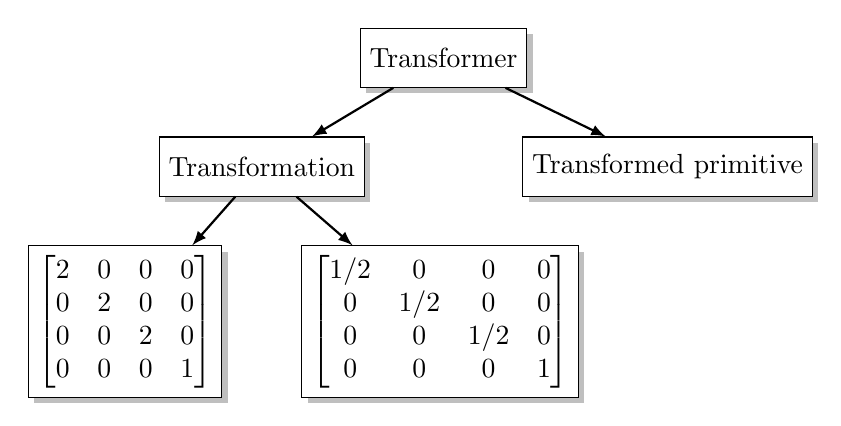
\begin{tikzpicture}[object/.style={draw,minimum height=.75cm,fill=white,drop shadow},arrow/.style={-latex,thick}]
  \node[object] (transformer) {Transformer};
  \node[object,anchor=north east] (transformation) at ($ (transformer) + (-1, -1) $) {Transformation};
  \node[object,anchor=north east] (matrix) at ($ (transformation) + (-0.5, -1) $) {
      $
        \begin{bmatrix}
          2 & 0 & 0 & 0 \\
          0 & 2 & 0 & 0 \\
          0 & 0 & 2 & 0 \\
          0 & 0 & 0 & 1 \\
        \end{bmatrix}
      $
    };
  \node[object,anchor=north west] (inverse matrix) at ($ (transformation) + (0.5, -1) $) {
      $
        \begin{bmatrix}
          1/2 & 0 & 0 & 0 \\
          0 & 1/2 & 0 & 0 \\
          0 & 0 & 1/2 & 0 \\
          0 & 0 & 0 & 1 \\
        \end{bmatrix}
      $
    };

  \node[object,anchor=north west] (primitive) at ($ (transformer) + (1,-1) $) {Transformed primitive};

  \draw[arrow] (transformer) -- (transformation);
  \draw[arrow] (transformation) -- (matrix);
  \draw[arrow] (transformation) -- (inverse matrix);
  \draw[arrow] (transformer) -- (primitive);
\end{tikzpicture}

\end{document}